\apendice{Especificación de Requisitos}

\section{Introducción}
En este apartado realizaremos un estudio de requisitos y objetivos que definirán el comportamiento del proyecto actual. También hablaremos de los diferentes casos de uso y los requisitos funcionales de la herramienta en cuestión.

\section{Objetivos generales}

Los objetivos generales que se quieren alcanzar al realizar este proyecto son los siguientes:
\begin{itemize}
	\item Implementar una página web para la realización de \textit{smart contracts}, en diferentes redes y con diferentes usuarios.
	\item Investigar las posibilidades y capacidades de conexión de la red ethereum y solidity para desarrollar \textit{smart contracts}.
\end{itemize}

\section{Catalogo de requisitos}

En este apartado mencionaremos los requisitos, divididos en funcionales y no funcionales.

\subsection{Requisitos funcionales}

\paragraph{RNF-1 Crear usuarios}: crear un sistema de gestión de usuarios y permisos para, así, garantizar la seguridad de la aplicación.

\paragraph{RNF-2 Actualizar usuario}: comprobación que permita la verificación de si el usuario o la contraseña fueron modificadas y desde qué cuenta realizó los cambios.

\paragraph{RNF-3 Eliminar usuario}: revisión para saber si el usuario fue borrado desde su propia cuenta o desde la cuenta de administrador.

\paragraph{RNF-4 Comprobar captha}: verificar el botón si pasa el proceso de no soy un robot.

\paragraph{RNF-5 Conexión con metamask}: al añadir producto, comprobar que pregunta si queremos conectar con dicha aplicación.

\paragraph{RNF-6 Creación del \textit{smart contracts}}: confirmar que el contrato  fue creado desde la página web a una red Ethereum mediante metamask.

\paragraph{RNF-7 Consultar productos}: podremos consultar todos los productos, tanto el ultimo añadido o todos en forma de tabla. También se incluye la hora de la creación del contrato. 

\paragraph{RNF-8 Salir de la aplicación}: funcionalidad que permita desconectar al usuario de la página web mediante un botón.

\subsection{Requisitos no funcionales}
\paragraph{RNF-1 Usabilidad}: la aplicación será intuitiva y fácil de utilizar, así como tener una una estructura clara para qué cualquier persona pueda comprenderla sin necesidad de ninguna formación.

\paragraph{RNF-2 Eficiencia}: la aplicación funcionará de una forma fluida, sin que la interfaz gráfica quede bloqueada.

\paragraph{RNF-3 Escalabilidad}: estará siempre abierta a la incorporación de nuevas funciones o programas.

\paragraph{RNF-4 Autonomía}: deberá realizar actualizaciones para no perder información y esta siempre intente ser la más fiable posible.

\section{Especificación de requisitos}

En esta sección podremos visualizar los casos de uso de los requisitos funcionales anteriormente explicados y también detallaremos todos los casos de uso mediante tablas.

\subsection{Diagramas de casos de uso}
En las siguientes figuras podremos observar los casos de uso que corresponden a nuestra aplicación, en la cual se podrán observar dos actores (administrador y usuario). Los UML los hemos realizado en la siguiente página web \cite{uml}

\begin{figure}[h!]
    \centering
    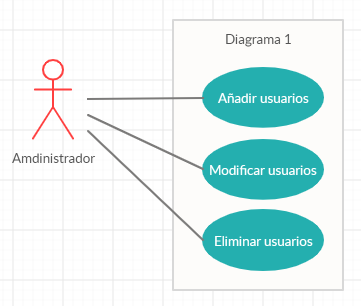
\includegraphics{CUAdmin}
    \caption{Diagrama de casos de uso del administrador}
\end{figure}

\imagen{CUUsuario}{Diagrama de casos de uso del usuario}

\subsection{Especificación de los casos de uso}

A continuación detallaremos mediante tablas los casos de uso:

\begin{table}[htbp]
	\begin{center}
		\begin{tabular}{|l|p{10cm}|}
		\hline
			\textbf{RF 1} & \textbf{Crear usuarios}                                                                                                                        			\\ \hline
			Descripción & Registro en la base de datos de nuevos usuarios.                                                                                                   \\ \hline
			Pre-condición & Un usuario deberá introducir un usuario, correo y una contraseña, con el objetivo de poder registrarse en la base de datos.\\ \hline
			Acción & Si el correo ya esta en uso, las contraseñas no coinciden o no marcamos la opción ``no soy un robot'', tendremos que repetir el proceso de registrarse. \\ \hline
			Post-condición  & Si el correo y la contraseña son correctos, nos mostrará la siguiente pantalla de la página Web.                                                     			\\ \hline
			Importancia & Alta                                                                                                                           \\ \hline
		\end{tabular}
	\caption{RF 1: Crear usuarios}
	\label{tabla:tablaB1}
	\end{center}
\end{table}

\begin{table}[htbp]
\begin{center}
\begin{tabular}{|l|p{10cm}|}
\hline
\textbf{RF 2} & \textbf{Actualizar usuario}                                                                                                                              \\ \hline
Descripción   & Dependiendo de si nos encontramos en un usuario o desde el administrador                                                                                 \\ \hline
Pre-condición   & Haber iniciado sesión previamente (desde administrador o de usuario).                                                                                    \\ \hline
Acción        & Podremos modificar el usuario y la contraseña de un usuario concreto, o, si estamos en el administrador, podremos acceder a modificar todos los usuarios. \\ \hline
Post-condición & Si todo fue correcto, los datos se modificarán en nuestra base de datos                                                                                  \\ \hline
Importancia   & Alta                                                                                                                                                     \\ \hline
\end{tabular}
\caption{RF 2: Actualizar usuarios}
	\label{tabla:tablaB2}
	\end{center}
\end{table}

\begin{table}[htbp]
\begin{center}
\begin{tabular}{|l|p{10cm}|}
\hline
\textbf{RF 3} & \textbf{Eliminar usuario}                                                                                                                       \\ \hline
Descripción   & Dependiendo de si nos encontramos en un usuario o desde el administrador, podremos ver o uno o a todos.                                         \\ \hline
Pre-condición   & Haber iniciado sesión previamente (desde administrador o de usuario).                                                                           \\ \hline
Acción        & Podremos eliminar el usuario de nuestra cuenta, ,o si estamos en el administrador, podremos acceder a eliminar los usuarios que deseemos.         \\ \hline
Post-condición & Si todo fue correcto, los datos se eliminarán en nuestra base de datos, también eliminaremos todos los productos que tiene adquiridos previamente. \\ \hline
Importancia   & Alta                                                                                                                                            \\ \hline
\end{tabular}
\caption{RF 3: Eliminar usuarios}
	\label{tabla:tablaB3}
	\end{center}
\end{table}

\begin{table}[htbp]
\begin{center}
\begin{tabular}{|l|p{10cm}|}
\hline
\textbf{RF 4} & \textbf{Comprobación captha}                                                                                                 \\ \hline
Descripción   & Cuando registramos un nuevo usuario, el ultimo apartado, una vez introducidos todos los campos, es demostrar que no se es un robot. \\ \hline
Pre-condición   & Ninguna                                                                                                                      \\ \hline
Acción        & Pulsar el botón no soy un robot, y seleccionar los campos que nos pida en cada momento.                                      \\ \hline
Post-condición & Si todo fue correcto, nos creará la nueva cuenta. \\ \hline
Importancia   & Alta                                                                                                                         \\ \hline
\end{tabular}
\caption{RF 4: Comprobar captha}
	\label{tabla:tablaB4}
	\end{center}
\end{table}

\begin{table}[htbp]
\begin{center}
\begin{tabular}{|l|p{10cm}|}
\hline
\textbf{RF 5} & \textbf{Conexión con metamask}                                                                                                                                                      \\ \hline
Descripción   & Realizar contrato desde la página web con la red Ethereum.                                                                                                                          \\ \hline
Pre-condición   & Haber iniciado sesión como usuario.                                                                                                                                                 \\ \hline
Acción        & Creación de un nuevo contrato cuando pulsamos ``Añadir Producto''. Si no tenemos Metamask conectado, nos saldrá una pantalla para iniciar sesión y crear el primer \textit{smart contracts} vacío. \\ \hline
Post-condición & Añadir todos los campos vacíos que se encuentran en la página web para la creación del \textit{smart contracts}.            \\ \hline
Importancia   & Alta                                                                                                                                                                                \\ \hline
\end{tabular}
\caption{RF 5: Conexión metamask}
	\label{tabla:tablaB5}
	\end{center}
\end{table}

\begin{table}[htbp]
\begin{center}
\begin{tabular}{|l|p{10cm}|}
\hline
\textbf{RF 6} & \textbf{Creación del \textit{smart contracts}}                                                                                                                                                            \\ \hline
Descripción   & Realizar contrato desde la página web con la red Ethereum.                                                                                                                                      \\ \hline
Pre-condición   & Haber iniciado sesión y estar en la página Añadir Producto.                                                                                                                                     \\ \hline
Acción        & Pulsaremos en ``Realizar contrato'' y nos saltará una notificación en metamask para confirmar o rechazar el contrato a realizar                                                                    \\ \hline
Pos-condición & Pulsar ``confirmar'' y tras una espera nos confirmará si se realizo correctamente pudiendo ver el contrato tanto en la red privada de Ropsten o consultando los productos añadidos de la página web. \\ \hline
Importancia   & Alta                                                                                                                                                                                            \\ \hline
\end{tabular}
\caption{RF 6: Creación del \textit{smart contracts}}
	\label{tabla:tablaB6}
	\end{center}
\end{table}

\begin{table}[htbp]
\begin{center}
\begin{tabular}{|l|p{10cm}|}
\hline
\textbf{RF 7} & \textbf{Consultar productos}                                                                                \\ \hline
Descripción   & Posibilidad de informarse de los productos que un usuario ha registrado en la red Ethereum.                 \\ \hline
Pre-condición   & Haber iniciado sesión y haber añadido un producto anteriormente (si no la página nos saldrá vacía).         \\ \hline
Acción        & Ir a la página de consulta de productos para poder observar los productos añadidos.                         \\ \hline
Post-condición & Podremos ver los productos que añadió cada usuario, solo podrán verse los productos del usuario registrado. \\ \hline
Importancia   & Alta                                                                                                        \\ \hline
\end{tabular}
\caption{RF 7: Consultar productos}
	\label{tabla:tablaB7}
	\end{center}
\end{table}

\begin{table}[h!]
\begin{center}
\begin{tabular}{|l|p{10cm}|}
\hline
\textbf{RF 8} & \textbf{Salir de la aplicación}                                \\ \hline
Descripción   & Cerrar sesión de nuestra página web.                           \\ \hline
Pre-condición   & Haber iniciado sesión.                                         \\ \hline
Acción        & Pulsar el botón de cerrar sesión, ubicado en su propio avatar. \\ \hline
Post-condición & Al cerrar sesión se desconectará de la pagina web.             \\ \hline
Importancia   & Alta                                                           \\ \hline
\end{tabular}
\caption{RF 8: Salir de la aplicación}
	\label{tabla:tablaB8}
	\end{center}
\end{table}
